%
% The first command in your LaTeX source must be the \documentclass command.
\documentclass[sigconf]{acmart}

\usepackage{graphicx}
\usepackage{float}

\sloppy


% Disable the extra information at the foot at first page for better viewing experience for a normal document.
\settopmatter{printacmref=false} % Removes citation information below abstract
\renewcommand\footnotetextcopyrightpermission[1]{} % removes footnote with conference information in first column
\pagestyle{plain} % removes running headers

%
% defining the \BibTeX command - from Oren Patashnik's original BibTeX documentation.
\def\BibTeX{{\rm B\kern-.05em{\sc i\kern-.025em b}\kern-.08emT\kern-.1667em\lower.7ex\hbox{E}\kern-.125emX}}

\begin{document}

\title{Project Proposal: \\ Study the knowledge flow into \textit{Stack Overflow} and from \textit{Stack Overflow} to \textit{GitHub}}

\author{Wenhan Zhu (Cosmos)}
\email{w65zhu@uwaterloo.ca}
\affiliation{%
  \institution{University of Waterloo}
  \city{Waterloo}
  \country{Canada}
}

% The abstract is a short summary of the work to be presented in the article.
\begin{abstract}

\textit{Stack Overflow} is the most popular Q\&A website about programming. \textit{Stack Overflow} contains large amount of public knowledge that should not be ignored. Many code snippets from answers on \textit{Stack Overflow} have been found in used by projects hosted on \textit{GitHub}. \textit{Stack Overflow} posts consists links to many other websites that can be considered as its sources. In this project we intend to find the knowledge flow of \textit{Stack Overflow} posts. 

In this project we explored what are the most popular source of references on \textit{Stack Overflow} and looked at how are \textit{Stack Overflow} code snippets reused on \textit{GitHub}. TODO: Results for RQ 2, 3, 4, 5

\end{abstract}

\keywords{\textit{Stack Overflow}, \textit{GitHub}}

\maketitle

\section{Introduction}

\textit{Stack Overflow}, since its introduction in 2011, has became the largest Q\&A website that focuses on programming. Due to the massive about of answer and questions on the website, there are large amount of public knowledge. Extracting and understanding these information on \textit{Stack Overflow} has been quite popular recently in the Software Engineering community. There has been numerous studies on \textit{Stack Overflow} focusing on different aspects. People are trying to understand how \textit{Stack Overflow} works and are trying to predict the quality answers on \textit{Stack Overflow}. Recently, a new database \textit{SOTorrent} based on the official \textit{Stack Overflow} datadump has been created.\cite{Baltes:2018:SRA:3196398.3196430} This dataset creates new opportunities to learn about \textit{Stack Overflow}

\textit{GitHub} is the largest code sharing website that hosts \textit{git} repositories. There are many code segments on \textit{GitHub} that originates from \textit{Stack Overflow} posts. There has been multiply efforts trying to study the effects of using \textit{Stack Overflow} code snippets on \textit{GitHub}. Previous studies has shown that code reuse on \textit{GitHub} from \textit{Stack Overflow} could cause security issues. \cite{7958574} 

In this project, we want to look at how information is shared to \textit{Stack Overflow} and how \textit{GitHub} projects reuses code snippets from \textit{Stack Overflow}. We will be trying to answer the following research questions.

\begin{enumerate}
	\item RQ1: What information are shared to \textit{Stack Overflow}
	\item RQ2: What projects reuses code from \textit{Stack Overflow}
	\item RQ3: Are \textit{Stack Overflow} code modified when used on \textit{GitHub} projects?
	\item RQ4: Does code snippets introduced from \textit{Stack Overflow} on \textit{GitHub} evolve over time?
	\item RQ5: Does updates to code snippets originated from \textit{Stack Overflow} on \textit{GitHub} triggers updates to the original post?
\end{enumerate}

The rest of this report is formatted as follows, Section 2 will talk about the background information and the dataset; Section 3 will answer the research questions; Section 4 is the conclusion; Section 5 is related work; Section 6 is threats to validity and Section 7 covers future work. Section 8 is the summary. 

\section{Background}
To understand the scope of this project, more details about the infrastructure of \textit{Stack Overflow} and \textit{SOTorrent} is needed. And some information about code clone is stated here.

\subsection{\textit{Stack Overflow}}

\subsubsection{\textit{Stack Overflow} official data dump}

In \textit{Stack Overflow}'s data dump, it contains information about all the posts and their history on the website. Other information such as comments in each post and the upvotes and downvotes to a post is also recorded.

In \textit{Stack Overflow} both the question and answer of considered as posts. Each post have a unique \textit{PostId} and their \textit{PostTypeId} determines whether they are a question post or an answer post. An answer post have a \textit{ParentId} that identifies the question they are answering. 

\subsubsection{\textit{SOTorrent}}

\textit{SOTorrent} is build on top of \textit{Stack Overflow} official data dump. In addition to the contents on \textit{Stack Overflow}'s official data dump. They analyzed the body of each \textit{Stack Overflow} post history and separated them into text and code blocks. Then they created a relationship between post versions so that studying the evolution of each block can be done easily. They also extracted every link in \textit{Stack Overflow} posts and comments and also queried the \textit{Google GitHub Dataset} to look for references of \textit{Stack Overflow} posts on \textit{GitHub}. These information made the study of this project possible. In this project, we are using the Dec. 2018 version of this dataset.

\subsection{\textit{GitHub dataset}}
\textit{Google GitHub Dataset} is public dataset that contains repositories from \textit{GitHub}. The documentation of this datasets seems to be lost on the internet, however, earlier blog posts on the subject suggests that this dataset mirrors code that have a clear open source license, ignores unchanged forks and un-notable projects such as empty projects. And it only contain files that are less then 10M. Some basic queries people ran suggests that it contains around 5\% of all the repositories. And as of June 2017, around 54\% of project with more than 15 stars are mirrors on the dataset. In the rest of the reports, data from \textit{GitHub} will mean data of \textit{GitHub} in this public dataset.

\subsection{Code Clones}
When a code snippets is reused on \textit{GitHub} projects, we want to understand how much it was modified. Research in code cloning has identified the type of code clone in 4 different ways. The definition are from \textit{Roy}'s work on comparing code clone tools. \cite{Roy:2009:CEC:1530898.1531101}

\textsc{TYPE-1} clone is a exact copy of the code besides white spaces, layout and comments.

\textsc{TYPE-2} clone is syntactically identical fragments except for variations in identifiers, literals, types and everything above.

\textsc{TYPE-3} clone is copied fragments with further modifications in addition to everything above. 

\textsc{TYPE-4} clone is two piece of code with same functionality but implemented differently.

Modern code clone tools are very good at {\sc TYPE-1, TYPE-2} clones but suffer to succeed in the later too. In this report, we will focus on TYPE-1 clones.

There are 3 major types of clone detection tool, text-based, token-based and tree-based. In this project we will be using basic token-based comparison on \textit{Python} code snippets.

\section{Code reuse on \textit{GitHub}}

For RQ3, Are \textit{Stack Overflow} code modified when reused on \textit{GitHub} projects, we want to study when \textit{Stack Overflow} code is referenced in \textit{GitHub} files, how much is modified. We limited our study on \textit{Python} files that have references to \textit{Stack Overflow} in this project. \textit{Python} has a built in lexical tokenize that can tokenize valid \textit{Python} code.

\subsection{Method}

There is a table in \textit{SOTorrent} that records all references to \textit{Stack Overflow} posts in files on \textit{Google GitHub Dataset}.  The table is extracted by matching a regular expression line by line on each file to check whether it matches a \textit{Stack Overflow} \textit{url}. This dataset as of Dec. 2018 is built soly from the data extracted from the files. The \textit{PostId} and \textit{PostTYpeId} are extracted from the \textit{url} extracted from individual files. Due to this reason, there contains many conflicting information on this dataset. Using this dataset, we extracted all references of \textit{Stack Overflow} posts of \textit{GitHub} files that have an extension of \textit{.py} which is a file extension for \textit{Python} files. This resulted in 126,244 unique references of \textit{Stack Overflow} posts for \textit{Python} files on \textit{GitHub}. We then filtered the results by its \textit{PostTypeId} to only have answer posts. By doing so, we only limit the references to exact answer posts so there is no ambiguity here about which exact post the file is referencing to. Due to the information was not verified with \textit{Stack Overflow} official dump, we cross verified the \textit{PostId} remaining with the official \textit{Stack Overflow} data dump to remove noise from the references. We then retrieved all the files from \textit{GitHub} and ignored files that were not retrievable. This resulted in 42,895 unique references to \textit{Stack Overflow} answer posts in \textit{Python GitHub} files. By manually looking at the files there we were not able to retrieve, we realized that these repositories were either deleted or turned in to private repositories between the version of \textit{SOTorrent} we are using, Dec. 2018, and the time of this project, Mar. 2019. 

In order to measure how much code was changed when introducing \textit{Stack Overflow} code segments to \textit{GitHub}, we need to define a metric for measuring the similarity. In this study we are using the token similarity defined as follows. Here, $S_{SO}, F_{GH}$ refers to the code segment on \textit{Stack Overflow} and the file on \textit{GitHub} that contains the reference to the post containing the code segment. $T$ is the tokenizing function that removes all formatting and style tokens such as line break, white spaces and comments. $MaxSubTokens$ calculates the maximum matching sub-token of 2 token lists and return the maximum matching sub-token. When dealing with tokens for \textit{Python} code, we matches the exact string from the token and not anything else.

$$
Sim(S_{SO}, F_{GH}) = \frac{|MaxSubTokens(T(S_{SO}), T(F_{GH}))|}{|T(S_{SO})|}
$$

For each reference we have, we extracted the code segments of the \textit{Stack Overflow} post by using a \textit{HTML parser}. This step was very straight forward due to posts in \textit{Stack Overflow} are written in \textit{Markdown} and every code segment are surrounded by \texttt{<code> some code segment </code>}. We then run the \textit{Python} tokenizer on each of the code segments of the post and compare it to the result of tokenizing the \textit{GitHub} file referencing this post. We ignored all reference if either the post does not contain any code segments or if the tokenizer fails on any of the code segments. To combat general matched tokens, we limited the minimum matched token length to be 40. Also, to make sure we are not double counting files in the same repository but different branches, we limited ourselves to the \texttt{master} branches.

This gave us a total of 3,490 references that matches our requirements. Some references have more then one code segment in the post that satisfies our constraints, we only consider the one with maximum similarity of all the code segments. This happens only to about 100 of the references. The method we are looking at code reuse from \textit{Stack Overflow} on \textit{GitHub} is by definition looking at \textsc{TYPE-1} clones of code. 

\subsection{Results}

\begin{figure}[h]
\centering
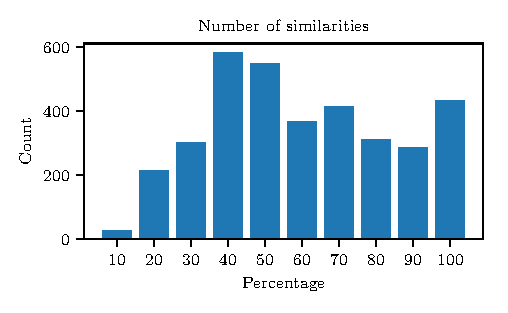
\includegraphics[width=\linewidth]{Figure_2.pdf}
\caption{Distribution of similarity percentage}
\label{fig:dis_sim}
\end{figure}

Figure \ref{fig:dis_sim} shows the distribution of percentage of similarities between \textit{Stack Overflow} posts and their references on \textit{GitHub}. The mean and median of the distribution are 55.00\% and 50.70\%.

The results show that on average, when a \textit{Stack Overflow} code snippet is reused on \textit{GitHub} projects, the maximum length of matching sub-token is a little more than the length of the tokens extracted from code segments. So when a reuse happens, on average at least half of the content remains unchanged. To further explored what are the popular changes, we manually looked at some of the references to have a better understanding. 

On \textit{Stack Overflow} many \textit{Python} code segments contain additional information about the modules they are importing. These import statements are often separated from the code segment in practice. So when matching the tokens between the two, we will lose similarity percentage due to not having these matched. Some other common reasons are adding statements and removing statements to better fit needs and changing the variable names to match the actual use. Modifying variable names can be taken care of if we move to a \textsc{TYPE-2} clone detection techniques. Detecting adding, removing statements are much harder. And taking care of the special cases of imports is very \textit{Python} specific, we think if the focus is only \textit{Python} snippets these can be treated, but in general it's very hard to deal with those language specific things.

So for RQ3, Are \textit{Stack Overflow} code modified when used on \textit{GitHub} projects, on average a specific code segments from \textit{Stack Overflow} reused on a \textit{GitHub} file contains a little more than half identical parts.

\section{Evolution of reused \textit{Stack Overflow} code snippets}

In RQ4, Does code snippets introduced from \textit{Stack Overflow} on \textit{GitHub} evolve over time, we want to see whether code snippets from \textit{Stack Overflow} on \textit{GitHub} are updated over time. 

\subsection{Method}

We took the final 3,490 reference that we find from the previous section and cloned the bare repository from \textit{GitHub}. There were 1 repository that was deleted between when we retrieved the files for the previous step and for this analysis, so we have 3,489 references to work with for this research question.

We first cloned the bare repository for \textit{GitHub} for each of the references. Then using the information from the maximum length sub-tokens of \textit{Stack Overflow} code segments and \textit{GitHub} files, we retrieved the number of lines that contained those tokens. Using this information, we were able to retrieve the history of these lines from the \textit{git} repository we retrieved from \textit{GitHub} by using \texttt{git log}.

The \texttt{git log} information we retrieved from the repositories gives the information of every commit that touches the aforementioned lines of code. It is also able to trace through the lines modified dynamically so that we will get all the information. The other popular command \texttt{git blame} can also do this, but it lacks the ability to recursively trace every commit that modified the lines specified.

\subsection{Results}

\begin{figure}[h]
\centering
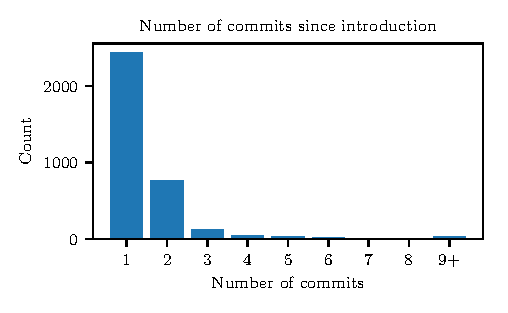
\includegraphics[width=\linewidth]{Figure_3.pdf}
\caption{Distribution of number of commits}
\label{fig:dis_commits}
\end{figure}

\begin{figure}[h]
\centering
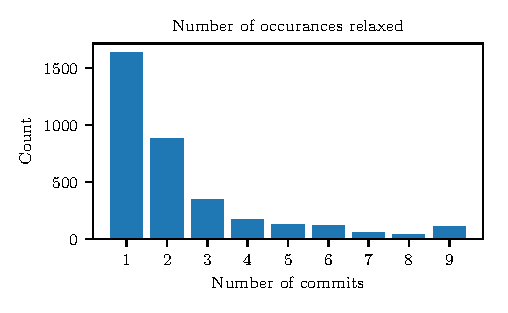
\includegraphics[width=\linewidth]{Figure_4.pdf}
\caption{Distribution of number of commits relaxed}
\label{fig:dis_commits_r}
\end{figure}


Figure \ref{fig:dis_commits} shows the distribution of number of commits for the 3,489 references we have looked at. The majority of the code segments never received an update after its introduction. Considering that the results from from the code segments that were matched with files of present and looked back for changes, it is likely that the modified code segments were not captured during token matching. So we retrieved another log with relaxed line numbers both 5 more lines before and after the starting and ending lines from the tokens. Figure \ref{fig:dis_commits_r} captures the distribution of number of commits regarding the relaxed lines.


So for RQ4, does code snippets introduced from \textit{Stack Overflow} on \textit{GitHub} evolve over time? Our results showed that code snippets reused on \textit{GitHub} does not get updated the majority of the time.


\section{Co-evolution of reused code snippets}

We investigate RQ5, does updates to code snippets originated from \textit{Stack Overflow} on \textit{GitHub} triggers updates to the original post, in this section. We want to understand whether changes to the code segments reused on \textit{GitHub} co-evolve with the original code snippet from \textit{Stack Overflow}.

\subsection{Method}
We took the references of \textit{Python} code snippets from the previous section and determined the date of the first commit that introduced the code segment from \textit{Stack Overflow}. We then extracted the number of edits for a post from \textit{Stack Overflow} data dump. Then we compared the time of each edit on \textit{Stack Overflow} and the earliest commit date of the code snippets on \textit{GitHub}.

\subsection{Results}

\begin{figure}[h]
\centering
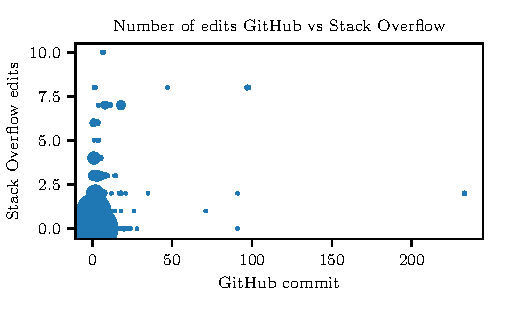
\includegraphics[width=\linewidth]{Figure_5.pdf}
\caption{Scatter plot for commits and edits}
\label{fig:ghsouc}
\end{figure}

Figure \ref{fig:ghsouc} is the scatter plot of the number of commits since introduction of code snippets on \textit{GitHub} and the number of edits to the \textit{Stack Overflow} post. Each data point is scaled based on the number of points at this location. Besides a few outliers, we can see that most of the code snippets does not get updates either on \textit{Stack Overflow} or \textit{GitHub}. The \textit{Pearson} correlation between the number of commits and edits is $0.2187$ with $p = 4.4 \ctimes 10^{-38}$. This shows that there exist only a weak to very weak correlation between commits on \textit{GitHub} code snippets from \textit{Stack Overflow} and the edits to the original post.

So for RQ5, updates to code snippets reused from \textit{Stack Overflow} on \textit{GitHub} generally does not trigger an edit to the original post.

\section{Related Research}

Since \textit{Stack Overflow}'s introduction, it has attracted many researchers to work on the subject. Some research wants to understand the model of \textit{Stack Overflow} \cite{Barua2014} and why it works with its gamification. \cite{Cavusoglu:2015:GMV:2685553.2698999} Interaction between \textit{Stack Overflow} and other platform has also been looked at. \textit{Vasilescu et al.} looked into common users between \textit{Stack Overflow} and \textit{GitHub}. They discovered that novice and experienced developer from \textit{GitHub} have different patterns of activity on \textit{Stack Overflow}. \cite{6693332}

There has also been research done to study how to improve \textit{Stack Overflow}. \textit{Duijn et al.} looked into prediction the quality of questions by looking at how many answers the question attracted. \cite{Duijn:2015:QQN:2820518.2820574} Previous study has shown that the number of answers of a question is highly correlated to the number of upvotes. Therefore, \textit{Dujin et al.} decided to use 2 answers (the mean of answers to \textit{Stack Overflow} posts) as a line for quality questions. \textit{Saha et al.} created a model to better predict tags for \textit{Stack Overflow} questions. \cite{Saha:2013:DMA:2487085.2487103} 

Researchers also use \textit{Stack Overflow} data to improve the development process of developers. \textit{Ponzanelli et al.} tried to mine \textit{Stack Overflow} for better IDE suggestions. \cite{Ponzanelli:2014:MST:2597073.2597077}

Mining \textit{Stack Overflow} has been really popular in recent years. The public knowledge from \textit{Stack Overflow} is very rich. \textit{Treude et al.} mined information from \textit{Stack Overflow} to augment API documentation. \cite{7886920} 

\section{Vulnerabilities}

\subsection{Threats to Validity}

Both the reference to and from \textit{Stack Overflow} in \textit{SOTorrent} are extracted by looking at \textit{HTML} links. So there could be referenced information but not present in the dataset. Also not every code reuse is referenced, for code reuse from \textit{Stack Overflow} to \textit{GitHub} we could look at site wise code clone detection but the scale will be enormous and unlikely to be possible due to the size of the corpus. There won't be any effective way off my mind how we would detect unreferenced sources to \textit{Stack Overflow}.

The source clone tool that is landed on could lead to problems. So I'll try my best to find the tool that serves the purpose will.

\subsection{Potential Problems}

In this case, the source code is required from \textit{GitHub}. Due to the API limits of \textit{GitHub} it's unsure whether acquiring the source code will be smooth. 

As a novice to databased and previous problems I've encountered with them. Having the dataset setup could also be more effort than expected. 

Having not used a source clone tool before, experimenting and setting up could have problems.

Time could also be a problem due to the scale of the project. However, I would like to answer most of the questions.


\bibliographystyle{ACM-Reference-Format}
\bibliography{sample}

\end{document}
